\section{高维最小绝对值回归的性能研究}
基于$L_1$范数的方法在宏观经济数据处理中的一个重要应用就是在建立线性模型时使用最小绝对值回归。在宏观经济实证研究中,经济变量往往
不能够服从正态分布,而因受到经济冲击呈现出重尾的特征。使用最小二乘法建立的线性回归模型虽然具有较好的解释性,
但是对原始数据的分布情况要求高,因此常常在回归中剔除异常点,使得经济变量接近正态分布,然而代价是有可能损失较多有价值的信息。
采用最小绝对值回归,是更加稳健的做法,实质上它就是中位数回归,也具有很好的解释性,可以很好处理重尾的宏观经济变量。

然而,应对高维宏观经济数据,最小绝对值回归由于需要解决高维线性规划问题,因此在计算的时间和空间复杂度都较高,
在一定程度上限制了它的应用。本章介绍了最小绝对值回归的主流估计方法,并介绍了两种性能较高的估计方法:1)基于聚类——迭代拆解的算法;
2)基于替代变量的牛顿迭代方法。通过模拟数值实验,验证了两种算法的高效性。

\subsection{简介}
\subsubsection{$L_1$范数的稳健性}

$L_2$范数最优化问题最常见的是最小二乘法。
最小二乘法的优点很多,这里不赘述。尽管在求解大部分问题时用最小二乘估计求解可以得到比较令人满意
的效果, 但最小二乘法也存在一些局限性, 比如, 当收集的数据较少或者具有较多的缺失数据
并且数据中夹杂有异常点时, 用最小二乘法所得的结果就令人难以接受, 在此情况下应用所得到到的回归方程或模型进行预测或者拟合时, 
则预测或拟合的精度是相当低的, 甚至根本不能使用。正因为最小二乘法对数据中的异常值十分敏感,当数据中具有较多离群值时,通过最小二乘、PCA和SVD方法,得到的估计结果也会受到较大影响。

这里可以不使用最小二乘法而选择$L_1$范数的方法即最小一乘法,它可以增加估计的健壮性。
设$\bm{X} = (X_1, X_2, ..., X_p)^T$为一$p$维随机变量,$Y$为响应变量,$\bm{\beta}$为回归系数。
假设我们观察到$i.i.d. $样本$\bm{X}_{n\times p} = (\bm{x}_1, \bm{x}_2, ..., \bm{x_n})^T$和$\bm{Y}_{n\times1}=
(y_1, ..., y_n)^T$,我们一般使用$\bm{\beta}$
的最小二乘估计量
\begin{equation}\label{l2loss}
\hat{\bm{\beta}} = \underset{\bm{\beta}}{\operatorname{arg\ min}} \sum_{i=1}^n\|y_i - \bm{x}^T_i\bm{\beta}\|_{L_2}
=\underset{\bm{\beta}}{\operatorname{arg\ min}} \sum_{i=1}^n(y_i - \bm{x}^T_i\bm{\beta})^2
\end{equation}
在稳健统计中,我们经常使用其他的目标函数,例如使用$L_1$范数来代替$L_2$,

\begin{equation}\label{l1loss}
\hat{\bm{\beta}} = \underset{\bm{\beta}}{\operatorname{arg\ min}} \sum_{i=1}^n\|y_i - \bm{x}^T_i\bm{\beta}\|_{L_1}
=\underset{\bm{\beta}}{\operatorname{arg\ min}} \sum_{i=1}^n|y_i - \bm{x}^T_i\bm{\beta}|
\end{equation}
如图所示,通常使用$L_1$范数在线性回归中可以有效避免离群值造成的干扰。
\begin{figure}[H]
    \centering
    \begin{minipage}[t]{0.48\textwidth}
    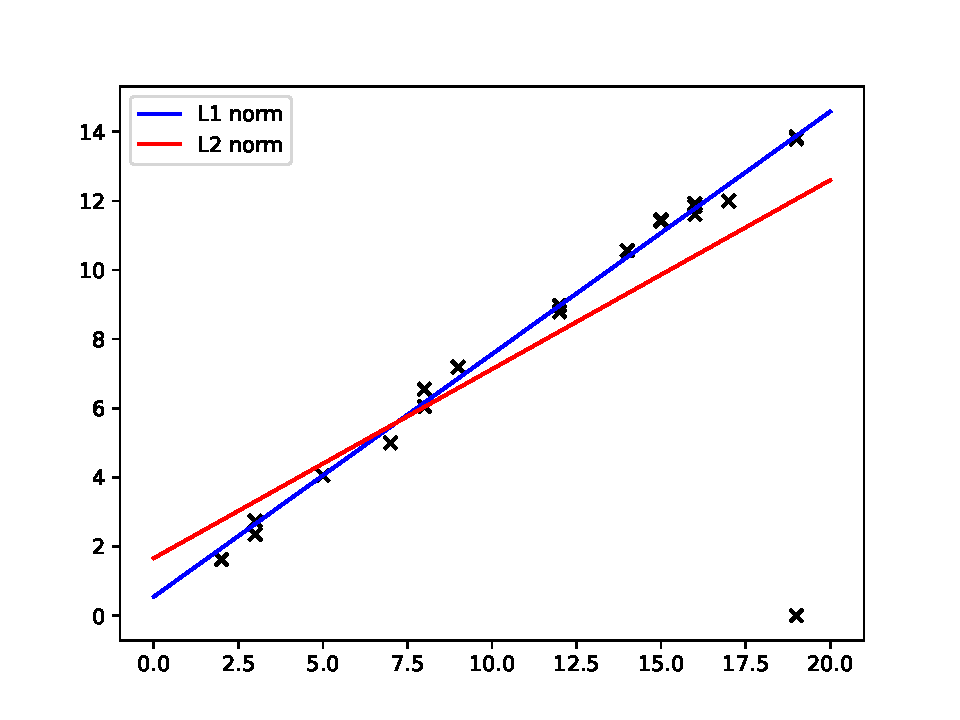
\includegraphics[width=8cm]{pics/l1-l2-diff2.pdf}
    \end{minipage}
    \begin{minipage}[t]{0.48\textwidth}
    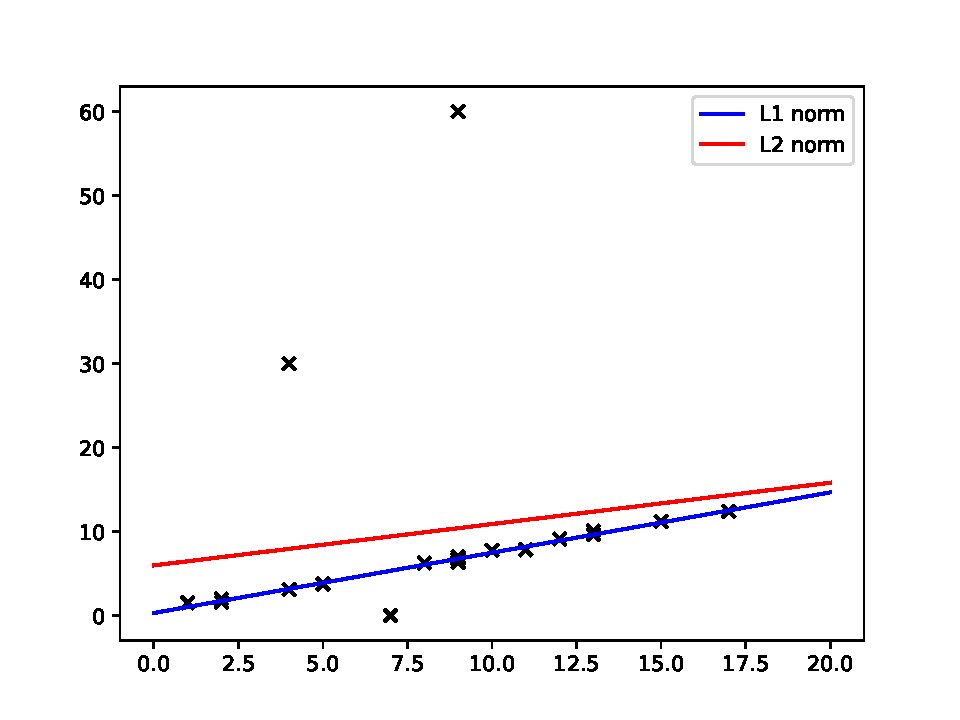
\includegraphics[width=8cm]{pics/l1-l2-diff.pdf}
    \end{minipage}
    \caption{\small 如图所示,在简单的线性模型的拟合中,出现一个离群值就可以导致最小二乘法拟合出现明显的偏差;
    而含有较多离群值时最小二乘法拟合变得很不可靠;而采用$L_1$范数则具有相当稳健性。}
    \label{fig2.1}

\end{figure}

\subsubsection{最小绝对值回归的估计方法}
对于\eqref{l1loss},它是一个凸优化问题,但是其不具备显式解,一般求它的数值解。但是其目标函数在$\bm{0}$点不可导,
因此不能直接使用使用梯度下降法,一般来说,该问题
的全局最优解可以通过求解下面的线性规划问题得到:
$$
    \underset{\bm{\beta}, \bm{t}}{\operatorname{min\ }} 1^T \bm{t}
$$
$$
    s.t. -\bm{t} \leq \bm{X}_{n\times p}\bm{\beta}_{p\times1} - \bm{Y}_{n\times 1} \leq \bm{t}
$$
目前对于线性规划问题已经有了比较成熟的解决方法,主要通过单纯形法或者内点法求解,后者的时间复杂度可以控制在多项式时间,
然而,一般而言,当$n$和$p$均很大时,上述线性规划问题面临很高的变量和约束维数,计算速度仍较慢。

由于$L_1$范数的目标函数在机器学习领域的大量使用,已经产生了一些光滑化方法,做法是用一个接近$L_1$的目标函数来替代它,
用来替代的函数往往处处可导,因而可以使用梯度下降法求解。
典型的代表就是使用Huber’s M统计量近似$L_1$范数目标函数,
\begin{equation*}
    \rho(e) = \left\{
        \begin{array}{clr}
            \frac1{2}e^2,\ |e| \leq \gamma \\
            \gamma |e| - \frac1{2}\gamma ^2 ,\ |e| > \gamma
        \end{array}
    \right.
\end{equation*}
其中$\gamma$为某一正数,该问题可以转化为一个二次规划问题求解。


\subsection{聚类——迭代拆解算法}
近年来针对最小绝对值回归的性能研究发展出了除了光滑化目标函数之外的方法,可以在不改变目标函数的情况下,
通过寻求新的优化方法进行求解。这样一来,可不改变最小绝对值回归估计量的统计性质。
这里介绍Park等人于2016年提出的一种基于聚类——迭代拆解算法的最小绝对值回归求解方法。


\subsubsection{聚类——迭代拆解算法说明}
聚类是一种在机器学习中常见的做法,就是按照某种给定的规则,将特征接近的样本点归类到一起。
聚类——迭代拆解算法的提出受到以下事实的启发:
1)优化问题规面临的数据集模庞大,其中许多的样本点在进行参数估计时的贡献是很接近的;
2)如果对相似的样本点进行聚类,只在每一类别中选则少量样本进入计算,那么就会大大减小问题的规模;
3)假设在聚类后构造的新数据集上不能接近问题的最优解,那么就拆解当前的聚类,
更换标准重新进行聚类,构造新的数据集;

采用聚类——迭代拆解算法求解某个优化问题的前提如下:1)必须能够提出一种规则来对样本点聚类;
2)必须找到合适的聚类和拆解聚类的标准;
3)需要在聚类后构造的新数据集上明确定义新的优化问题;
4)能够判定当前解是否接近最优解。

算法2.1给出了任何一个聚类——迭代拆解算法的主要步骤,注意算法2.1必然在某处停止,
因为每次不断拆解聚类,当聚类个数$|K^{t}|= n$时,相当于计算原问题,此时算法终止。
\begin{table}[H]%%%%%%开始表格
    \centering%把表居中
    \begin{tabular}{{p{0.9\columnwidth}}}%三个c代表该表一共三列,内容全部居中
    
    \toprule%第一道横线 表头
    算法2.1:聚类——迭代拆解算法(Aggregate and Iterative Disaggregate, AID) \\
    \midrule%第二道横线 符号+解释+单位 中间用&隔开
    输入:原始数据集$\bm{X}_{n\times p}$,样本点的下标集合${I} = \{1, 2, ..., n\}$,
    数据的特征下标集合${J} = {1, 2, ..., p}$,原优化问题$P$。\\
    初始化:对原始数据集$\bm{X}$聚类,然后按某种规则产生新的优化数据集$\bm{X}^{1}$。 \\
    对于$t = 1, ..., T$:\\
        记${C}^{t} = \{{C}_1^{t}, ..., C_K^{t}\}$为聚类的集合, $K^t = {1, ..., |K^t|}$为当前聚类的下标,
        \\
        1.根据当前聚类情况${C}^{t}$,构造新的数据集$\bm{X}^{t}$,求解相应的优化问题${P}^{t}$; \\
        2.检查解$\bm{s}^{t}$是否达到最优条件;\\
        3.如果不满足条件,拆解当前聚类。
        \\
    \bottomrule%第三道横线
    \end{tabular}
\end{table}%%%%%%结束表格

\subsubsection{解决最小绝对值回归问题}
改写\eqref{l1loss}的目标函数,
\begin{equation}\label{l1loss2}
E^* = \underset{\bm{\beta} \in \mathbb{R}^{p}}{\operatorname{min}} 
\sum_{i \in I}|y_i - \sum_{j \in J}x_{ij}\bm{\beta}_j|
\end{equation}

首先给出聚类方法。给定$|K_0|$为目标聚类个数,初始化$C_0 = \{C_1^0, C_2^0, ..., C_K^0\}$,
我们可以使用任意的聚类方法进行初始化。接下来给出如何根据聚类来产生新的数据集,
对于在任一迭代周期内产生的聚类$C^t_k, k = 1, ..., K^t$,取
\begin{equation*}
    x_{kj}^t = \frac{\sum_{i \in C_k^t}x_{ij}}{|C_k^t|},\ j \in J \  
    \text{并且} \
    y_{k}^t = \frac{\sum_{i \in C_k^t}y_i}{|C_k^t|}
\end{equation*}

对于每一个不同的聚类需要给出一个权重来区分信息量不同的聚类,因此在新的数据集上,我们求解下面的问题
\begin{equation}\label{clusterl1}
    F^t =\underset{\bm{\beta}^t \in \mathbb{R}^{p}}{\operatorname{min}} 
    \sum_{k=1}^{K^t}|C_k^t||y_k^t - \sum_{j \in J}x_{kj}^t\bm{\beta}_j^t|
\end{equation}
容易发现,任何\eqref{clusterl1}的可行解都是\eqref{l1loss2}的可行解。
记$\hat{\bm{\beta}^t}$为\eqref{clusterl1}的解,在每次迭代,我们计算此时的原目标函数的取值
\begin{equation}
    E^t = \sum_{i \in I} |y_i - \sum_{j \in J}x_{ij}\hat{\bm{\beta}}_j^t|
\end{equation}

接下来给出拆解聚类的准则:设$t$步的聚类集合为$C^{t}$,该步解为$\hat{\bm{\beta}}_t$,
对于$k = 1, ..., K^t$,计算$\theta_i = y_i - \sum_{j \in J}x_{ij}\hat{\bm{\beta}}_j^t$,
1)若对于任意$i \in C_k^t$,$\theta_i$有相同的符号,那么该聚类$C^t_k$将保留到下次迭代,即$C^{t+1} \leftarrow C^{t+1}\bigcup C^t_k$;

2)若不满足上述条件,那么根据$\theta_i$符号异同,将$C^t_k$分成两个集合,$C_{k+}^t = \{i \in C_k^t | \theta_i > 0\}$ ,
$C_{k-}^t = \{i \in C_k^t | \theta_i < 0\}$,这两个集合在下一步形成新的聚类,
即$C^{t+1} \leftarrow C^{t+1}\bigcup \{ C_{k+}^t, C_{k-}^t\}$。

结合算法2.1,到这里已经给出了完成聚类——迭代拆解最小绝对值回归的所有计算步骤,当聚类无法继续划分时,迭代终止。

下面证明最后一次迭代的解$\hat{\bm{\beta}}_j^T$就是\eqref{l1loss2}的解$\bm{\beta}^*$,
\begin{equation*}
    \begin{split}
        E^* & = \sum_{i \in I} |y_i - \sum_{j \in J}x_{ij}\bm{\beta}j^*|
        = \sum_{k \in K_t}\sum_{i \in C_k^t}|y_i - \sum_{j \in J}x_{ij}\beta_j^*| \\
        & \geq \sum_{k \in K^t}|\sum_{i\in C_k^t}y_i - \sum_{j \in J}x_{ij}\bm{\beta}_j^*|
        = \sum_{k \in K^t}|C_k^t||y_k^t - \sum_{j \in J}x_{kj}^t\bm{\beta}_j^*|\\
        & \geq \sum_{k \in K^t} |C_k^t||y_K^t - \sum_{j\in J}x_{kj} \hat{\bm{\beta}}_j^t|
        = \sum_{k \in K^t} |\sum_{i \in C_k^i} yi - \sum_{i \in C_k^t}\sum_{j \in J}x_{ij}\hat{\bm{\beta}}_j^t| \\
        & = \sum_{k \in k^t} \sum{i \in C_k^i}|y_i - \sum_{j \in J}x_{ij}\hat{\bm{\beta}}_j^t|
        = \sum_{i \in I}|y_i - \sum_{j \in J} x_{ij} \hat{\bm{\beta}}_j^t| 
        = E^t
    \end{split}
\end{equation*}

因为$\hat{\bm{\beta}}_t$是\eqref{l1loss2}的可行解,又显然$E^* \leq E^t$,
这就证明了$E^* = E^t$,注意到$ \sum_{k \in K^t} |C_k^t||y_K^t - \sum_{j\in J}x_{kj} \hat{\bm{\beta}}_j^t|$
就是$F^t$,因此$E^t = F^t$。因此最后一次迭代$F^T$的最优解$\hat{\bm{\beta}}_j^T$就是原问题的最优解。


\subsection{基于替代变量最小二乘的方法}

首先我们再次观察式($2-10$),
$$
    f_j = \underset{\theta}{\operatorname{arg\ min}} |A^{(t-1)}\theta - x_j|
$$
其中$x_j$为$p$维向量,因而目标函数可以改写成
$$
    |A^{(t-1)}\theta -x_j| = \sum_{i=1}^{p}|A^{(t-1)}_i \theta - x_{ji}| 
    = \sum_{i=1}^{p}\rho(A^{(t-1)}_i \theta - x_{ji})
$$
其中$\rho(x) = x(0.5 - \mathbb{I}[x \leq 0])$,
$\mathbb{I}(x)$为指示函数。$A_i^{(t-1)}$为矩阵$A^{(t-1)}$的第i行。
即
$$
    f_j =  \underset{\theta}{\operatorname{arg\ min}} \sum_{i=1}^{p}\rho(A^{(t-1)}_i \theta - x_{ji}) 
    \eqno{(3-1)}
$$

考虑如下线性回归问题:
$$ Y = \bm{X}^T\bm{\beta}^* + e$$
其中$\bm{X} = (\bm{X}_1, \bm{X}_2, ..., \bm{X}_{p+1})^T$为$p+1$维随机变量,$\bm{\beta}^* = (\bm{\beta}_0,\bm{\beta}_1, ..., \bm{\beta}_p)^T$为
回归系数,$Y$为响应变量,$e$为独立于$\bm{X}$的噪声。
假设我们使用$L_1$损失函数来估计$\bm{\beta}$,
$$\bm{\beta}^* = \underset{\bm{\beta} \in \mathbb{R}^{p+1}}{\operatorname{arg\ min}}\mathbb{E}|Y - \bm{X}^T\bm{\beta}| = 
\underset{\bm{\beta} \in \mathbb{R}^{p+1}}{\operatorname{arg\ min}}\mathbb{E}\rho(Y - \bm{X}^T\bm{\beta})
\eqno{(3-2)}
$$
若已知n\ $i.i.d.$ 的样本$(\bm{X}_i, Y_i)\ (1 \leq i \leq n)$,令$\hat{\bm{\beta}}$为$\bm{\beta}^*$的估计量,则
$$
    \hat{\bm{\beta}} = \underset{\bm{\beta} \in \mathbb{R}^{p+1}}{\operatorname{arg\ min}}\frac1{n}\sum_{i=1}^{n}\rho(Y_i - \bm{X}_i^T\bm{\beta})
    \eqno{(3-3)}
$$
可以发现式($3-3$)与($3-1$)有相同的问题形式,因此我们不妨考虑换一种方法估计$\bm{\beta}^{*}$,用新的估计量来代替$\hat{\bm{\beta}}$。

我们使用牛顿迭代法求解下面的随机优化问题:
$$
    \bm{\beta}^* = \underset{\bm{\beta} \in \mathbb{R}^{p+1}}{\operatorname{arg\ min}} \mathbb{E}[G(\bm{\beta};\bm{X},Y)]
    \eqno{(3-4)}
$$
其中$G(\bm{\beta};\bm{X}, Y)$是损失函数,$\bm{X}$和$Y$分别是$p+1$维自变量和一元响应变量,$\bm{\beta}$为回归系数。使用牛顿-拉弗森迭代来求解,
$$
    \tilde{\bm{\beta}}_1 = \bm{\beta}_0 - \bm{H}(\bm{\beta}_0)^{-1}\mathbb{E}[g(\bm{\beta};\bm{X},Y)]
    \eqno{(3-5)}
$$
其中$\bm{\beta}_0$是一个初始估计,$g(\bm{\beta};\bm{X},Y)$为损失函数$G(\bm{\beta};\bm{X},Y)$关于$\bm{\beta}$的梯度。\\
$\bm{H}(\bm{\beta}):=\partial\mathbb{E}[g(\bm{\beta};\bm{X},Y)
/\partial\bm{\beta}$表示$\mathbb{E}G(\bm{\beta};\bm{X},Y)$的海赛矩阵。特别地,我们这里考虑损失函数为$L_1$损失的特殊情形,
$$
    G(\bm{\beta};\bm{X},Y) = \rho(Y - \bm{X}^T\bm{\beta})
    \eqno{(3-6)}
$$
在($3-6$)的条件下,$g(\bm{\beta};\bm{X},Y) = \bm{X}(\mathbb{I}[Y - \bm{X}^T\bm{\beta} < 0] - 0.5)$。\\
并且,$\bm{H}(\bm{\beta}) = \mathbb{E}(\bm{X}\bm{X}^Tf(\bm{X}^T(\bm{\beta} - \bm{\beta}^*)))$,这里
$f(x)$是噪声$e$的密度函数。当初始估计量$\bm{\beta}_0$和$\bm{\beta}^*$很接近时,$\bm{H}(\bm{\beta}_0)$就会很接近
$\bm{H}(\bm{\beta}^*) = \bm{\Sigma}f(0)$,这里$\bm{\Sigma} = \mathbb{E}\bm{X}\bm{X}^T$是$\bm{X}$的协方差
矩阵。使用$\bm{H}(\bm{\beta}^*)$替换式($3-5$)中的$\bm{H}(\bm{\beta}_0)$,可得
$$
    \bm{\beta}_1 = \bm{\beta}_0 - \bm{H}(\bm{\beta}^*)^{-1}\mathbb{E}[g(\bm{\beta};\bm{X}, Y)]
    = \bm{\beta}_0 - \bm{\Sigma}^{-1}f^{-1}(0)\mathbb{E}[g(\bm{\beta}_0;\bm{X},Y)]
    \eqno{(3-7)}
$$
我们在$\bm{\beta}^*$对$\mathbb{E}[g(\bm{\beta}_0;\bm{X},Y)$进行泰勒展开,
\begin{equation*}
    \begin{split}
\mathbb{E}[g(\bm{\beta}_0;\bm{X},Y) &= \bm{H}(\bm{\beta}^*)(\bm{\beta}_0 - \bm{\beta}^*) + O(|\bm{\beta}_0 - \bm{\beta}^*|_2^2) \\
 &= \bm{\Sigma}f(0)(\bm{\beta}_0 - \bm{\beta}^*) + O(|\bm{\beta}_0 - \bm{\beta}^*|_2^2)
    \end{split}
\end{equation*}
结合式($3-7$),可以得到
\begin{equation*}
    \begin{split}
        |\bm{\beta}_1 - \bm{\beta}^*|_2 &=  |\bm{\beta}_0 - \bm{\Sigma}^{-1}f^{-1}(0)(
            \bm{\Sigma}f(0)(\bm{\beta}_0 - \bm{\beta}^*) + O(|\bm{\beta}_0 - \bm{\beta}^*|_2^2)
        ) - \bm{\beta}^*|_2\\
        &= O(|\bm{\beta}_0 - \bm{\beta}^*|_2^2)
    \end{split}
\end{equation*}
因此,如果我们得到一个$\bm{\beta}^*$的一致估计量$\bm{\beta}_0$,我们就可以通过式($3-7$)中的牛顿-拉弗森迭代得到
偏误更小的估计。

下面我们将($3-7$)转化成一个最小二乘问题。首先我们重写该式,
\begin{equation*}
    \begin{split}
    \bm{\beta}_1 &= \bm{\Sigma}^{-1}(\bm{\Sigma}\bm{\beta}_0 - f^{-1}(0)\mathbb{E}[g(\bm{\beta}_0;\bm{X},Y)])\\
    &= \bm{\Sigma}^{-1}\mathbb{E}[\bm{X}\{\bm{X}^T\bm{\beta}_0 - f^{-1}(0)(\mathbb{I}[Y \leq \bm{X}^T\bm{\beta}_0] - 0.5)\}]
    \end{split}
\end{equation*}
这里我们定义一个新的响应变量$\tilde Y$,
$$
    \tilde Y = \bm{X}^T\bm{\beta}_0 - f^{-1}(0) (\mathbb{I}[Y \leq \bm{X}^T\bm{\beta}_0] - 0.5)
$$
那么$\bm{\beta}_1 = \bm{\Sigma}^{-1}\mathbb{E}(\bm{X}\tilde{Y})$就是线性回归问题$\tilde Y = \bm{X}^T\bm{\beta}$
的最优回归系数,即
$$
    \bm{\beta}_1 = \underset{\bm{\beta} \in \mathbb{R}^{p+1}}{\operatorname{arg\ min}} 
    \mathbb{E}(\tilde Y - \bm{X}^T \bm{\beta})^2
$$

假设我们获得了$i.i.d.$样本$(\bm{X}_i, Y_i)$,则构造
$$
    \tilde{Y}_i = \bm{X}_i^T\hat{\bm{\beta}}_0 - \hat{f}^{-1}(0)
    (\mathbb{I}[Y_i \leq \bm{X}_i^T \hat{\bm{\beta}}_0] - 0.5)
$$
其中$\hat{\bm{\beta}}_0$为$\bm{\beta}^*$的一个初始估计,$\hat{f}(0)$为$f(0)$的一个估计,那么在牛顿迭代的每一步骤,
$$
    \hat{\bm{\beta}} = \underset{\bm{\beta} \in \mathbb{R}^{p+1}}{\operatorname{arg\ min}}
    \frac1{n} \sum_{i=1}^n(\tilde{Y}_i - \bm{X}_i^T\bm{\beta})^2
$$
这里我们选择最小二乘估计量作为$\hat{\bm{\beta}}_0$,并且采用$f(0)$的核密度估计作为$\hat{f}(0)$,
$$
    \hat{\bm{\beta}}_0 = \underset{\bm{\beta} \in \mathbb{R}^{p+1}}{\operatorname {arg\ min}}
    \frac1{n} \sum_{i=1}^n(Y_i - \bm{X}_i^T\bm{\beta})^2
$$
$$
    \hat{f}(0) = \frac1{nh}\sum_{i=1}^nK(\frac{Y_i - \bm{X}^T_i\hat{\bm{\beta}}_0}{h})
$$
其中$K(x)$为高斯核函数,$h \rightarrow 0$是带宽。

\begin{table}[H]%%%%%%开始表格
    \centering%把表居中
    \begin{tabular}{{p{0.9\columnwidth}}}%三个c代表该表一共三列,内容全部居中
    
    \toprule%第一道横线 表头
    算法2 使用牛顿-拉弗森迭代计算$L_1$最小化问题\\
    \midrule%第二道横线 符号+解释+单位 中间用&隔开
    输入:$Y$和$\bm{X}$的样本$\bm{Y} = (Y_1, Y2, ..., Y_n)$,$\bm{X} = (\bm{X}^T_1, \bm{X}^T_2, ..., \bm{X}^T_n)$,
    迭代次数$t$,高斯核函数$K$,带宽$h_g(g = 1, ..., t)。$
    \\
    初始化:给出$$\hat{\bm{\beta}}^{(0)} = \underset{\bm{\beta} \in \mathbb{R}^{p+1}}{\operatorname{arg\ min}}
    \frac1{n}\sum_{i=1}^n (Y_i - \bm{X}_i^T\bm{\beta})^2$$
    \\
    对于$g = 1, ..., t$:
    \\
        1. 计算$\hat{f}^{(g)}(0)$,
        $$
        \hat{f}^{(g)}(0) = \frac1{nh}\sum_{i=1}^{n}K(\frac{Y_i - \bm{X}_i^T\hat{\bm{\beta}}^{(g-1)}}{h_g})
        $$
    \\
        2. 计算$\tilde{Y} = (\tilde Y_1, \tilde Y_2, ..., \tilde Y_n)$,
        $$
        \tilde{Y}_i = \bm{X}^T_i\hat{\bm{\beta}}^{(g-1)} - \hat{f}^{(g)}(0)^{-1}
        (\mathbb{I}[Y_i \leq \bm{X}_i^T \hat{\bm{\beta}}^{(g-1)}] - 0.5)
        $$
    \\
        3. 计算$\hat{\bm{\beta}}^{(g)}$,
        $$
        \hat{\bm{\beta}}^{(g)} = \underset{\bm{\beta} \in \mathbb{R}^{p+1}}{\operatorname{arg\ min}}
        \frac1{n}\sum_{i=1}^n (\tilde{Y}_i - \bm{X}_i^T\bm{\beta})
        $$
    \\
    输出:$\bm{\beta}^{(t)}$
    \\
    \bottomrule%第三道横线
    \end{tabular}
\end{table}%%%%%%结束表格


\subsection{模拟实验}
\subsubsection{数据准备}


\subsection{本章小结}